\documentclass[11pt,a4paper]{jarticle}
\usepackage[dvipdfmx]{graphicx}
\usepackage{url}

\renewcommand{\baselinestretch}{1.05} 
\marginparwidth=0cm
\topmargin=-1cm
\headheight=0.3cm
\headsep=0.7cm
\oddsidemargin=0cm
\evensidemargin=0cm
%\textwidth=43zw
\textwidth=15.92cm
%\textheight=43.3\baselineskip
\baselineskip = 0.5744cm
\textheight=43\baselineskip

\itemsep=0.05\baselineskip
\parsep=0pt
\topsep=0.01\baselineskip
\partopsep=0pt
\listparindent=0zw

%% header and footer
\usepackage{fancyhdr}
\pagestyle{fancy}
\lhead{2014年度 春学期授業}
\chead{インタラクティブ・アート実習}
\rhead{担当教員: 松下 光範}
\cfoot{\thepage}
\renewcommand{\headrulewidth}{0pt}
\renewcommand{\footrulewidth}{0pt}

\usepackage{ascmac}
\usepackage{listings,jlisting}
\usepackage{color}
\definecolor{OliveGreen}{cmyk}{0.64,0,0.95,0.40}
\definecolor{colFunc}{rgb}{1,0.07,0.54}
\definecolor{CadetBlue}{cmyk}{0.62,0.57,0.23,0}
\definecolor{Brown}{cmyk}{0,0.81,1,0.60}
\definecolor{colID}{rgb}{0.63,0.44,0}
\definecolor{rulesepcolor}{gray}{0.666}
\lstset{
  language=Java,%プログラミング言語によって変える。
  basicstyle={\ttfamily\small},
  keywordstyle={\color{OliveGreen}},
  %[2][3]はプログラミング言語によってあったり、なかったり
  keywordstyle={[2]\color{colFunc}},
  keywordstyle={[3]\color{CadetBlue}},%
  commentstyle={\color{Brown}},
  %identifierstyle={\color{colID}},
  stringstyle=\color{blue},
  tabsize=2,
  %frame=trBL,
  %numbers=left,
  numberstyle={\ttfamily\small},
  breaklines=true,%折り返し
  %backgroundcolor={\color[gray]{.95}},
  framexleftmargin=0mm,
  frame=single,
  rulesepcolor=\color{rulesepcolor},
  captionpos=b
}


%%%%%%%%%%%%%%%%%%%%%%%%%%%%%%%%%%%%%%%%%%%%%%%%%%%%%%%%%%%%%%%%
\begin{document}

% title
\section*{\LARGE{第6講 応用編: 赤外線センサとモーターを連携させる}}
赤外線センサを用いて、センサと物体との距離を測定する。

モーターの回転速度を制御する。

測定した距離に応じてモータの回転数を制御する。

%%%%%%%%%%%%%%%%%%%%%%%%%%%%%%%%%%%%%%%%%%%%%%%%%%%%%%%%%%%%%%%%

\section{赤外線センサを用いて距離を測る}
物体との距離を非接触で測定するための方式には「超音波方式」と「赤外線方式」があります。
赤外線センサは、(その名の通り)赤外線を用いて距離を測定しています。
超音波センサは、物体から人体まで幅広いものの距離を検出することができる。

今回利用する赤外線センサは、大体 10cm 〜 80cm までの距離を測定することができます。
赤外線センサは、外光による影響を受けやすいため、使用する環境によっては注意する必要があります。
赤外線センサよりも、もう少し長い距離を測定したい場合は、超音波センサを使うと良いでしょう。

% 赤外線センサの図と配線の説明を入れる

\begin{itembox}[l]{注意!}
 赤外線センサは、とてもデリケートで配線の向きを間違えただけでも破損してしまいます。
 PC に接続する前に配線が正しいかどうか、もう一度確認すること!
\end{itembox}

\subsection*{回路}
% \begin{figure}[h!]
%  \centering
%  \includegraphics[width=\columnwidth]{img/ir_sensor.eps}
%  \caption{赤外線センサを用いた回路図}
% \end{figure}


\subsection*{プログラム}
光センサを圧力センサに置き換えたときのように、プログラムは同じものが使えます。
\begin{lstlisting}
 import processing.serial.*;
 import cc.arduino.*;
 
 Arduino arduino;
 int sensorPin = 0;
 PFont font;
 
 void setup() {
   size(300, 300);

   arduino = new Arduino(this, Arduino.list()[0]); 
   font = loadFont("Serif-48.vlw"); // Create Fontを忘れずに!
 }

 void draw() {
   background(255);

   int val = arduino.analogRead(sensorPin);

   textFont(font, 32);
   fill(0);
   text("val: " + val, 32, 32);
 }
\end{lstlisting}


\section{センサの値を実際の距離にマッピングする}
距離センサと後述する map 関数を組み合わせると、電子ものさしを作ることができます。

\subsection*{準備}
距離センサの値を取得して、数値がどのように変化するのか観察してみましょう。
また、センサの値が実際の距離とどのように対応付いているのをメモしておいてください。

% \subsection*{map関数}
% Processing には map 関数という機能が用意されています。
% 説明入れて
% 例えば、
% \begin{lstlisting}
%  float y = map(x, 0, 255, yMin, yMax);
% \end{lstlisting}
% map 関数は非常に便利なので覚えておくとよいでしょう。

% これ、意味わかるかな?
\begin{lstlisting}
 void draw() {
   background(255);

   int val = arduino.analogRead(sensorPin);

   // 距離が
   // 10cmのとき、センサの値が256で
   // 80cmのとき、センサの値が768の場合
   float distance = map(val, 255, 768, 10, 80);

   textFont(font, 32);
   fill(0);
   text(" val: " + val, 32, 32);
   text("dist: " + dist, 32, 64);
 }
\end{lstlisting}



\section{モーターを回転速度を制御する}
モーターを制御する回路にはいくつか種類がありますが、今回は配線が簡単な電界効果トランジスタ (FET: Field effect transistor) を使用した回路を用います。
モーターを回転させるには、比較的大きな電流が必要なため、Arduino の出力だけでは、モータを回転させ続けるパワーが足りません。
そのため、外部電源からモーターに電力を供給し、Arduino や Processing で制御するために必要となるのが FTE である。
FET を用いることで、モーターに流す電流を制御し、モーターの回転数を変化させることができます (電流が多く流れると早く回る)。


今回はいつもよりも多くの電子部品を使います。
それぞれ各自、以下の部品が手元にあるか、確認してください。
\begin{itemize}
 \item モーター(RE-140RA) 1個
 \item FET (2SK2232) 1個
 \item 赤外線距離センサ 1個
 \item 抵抗器(10kΩ) 1個
 \item 単4型乾電池 2個
 \item 電池ケース 1個
 \item ダイオード 1個
\end{itemize}
% 一つ一つ画像を入れたほうが良さそう

\subsection*{回路}
\begin{figure}[h!]
 \centering
 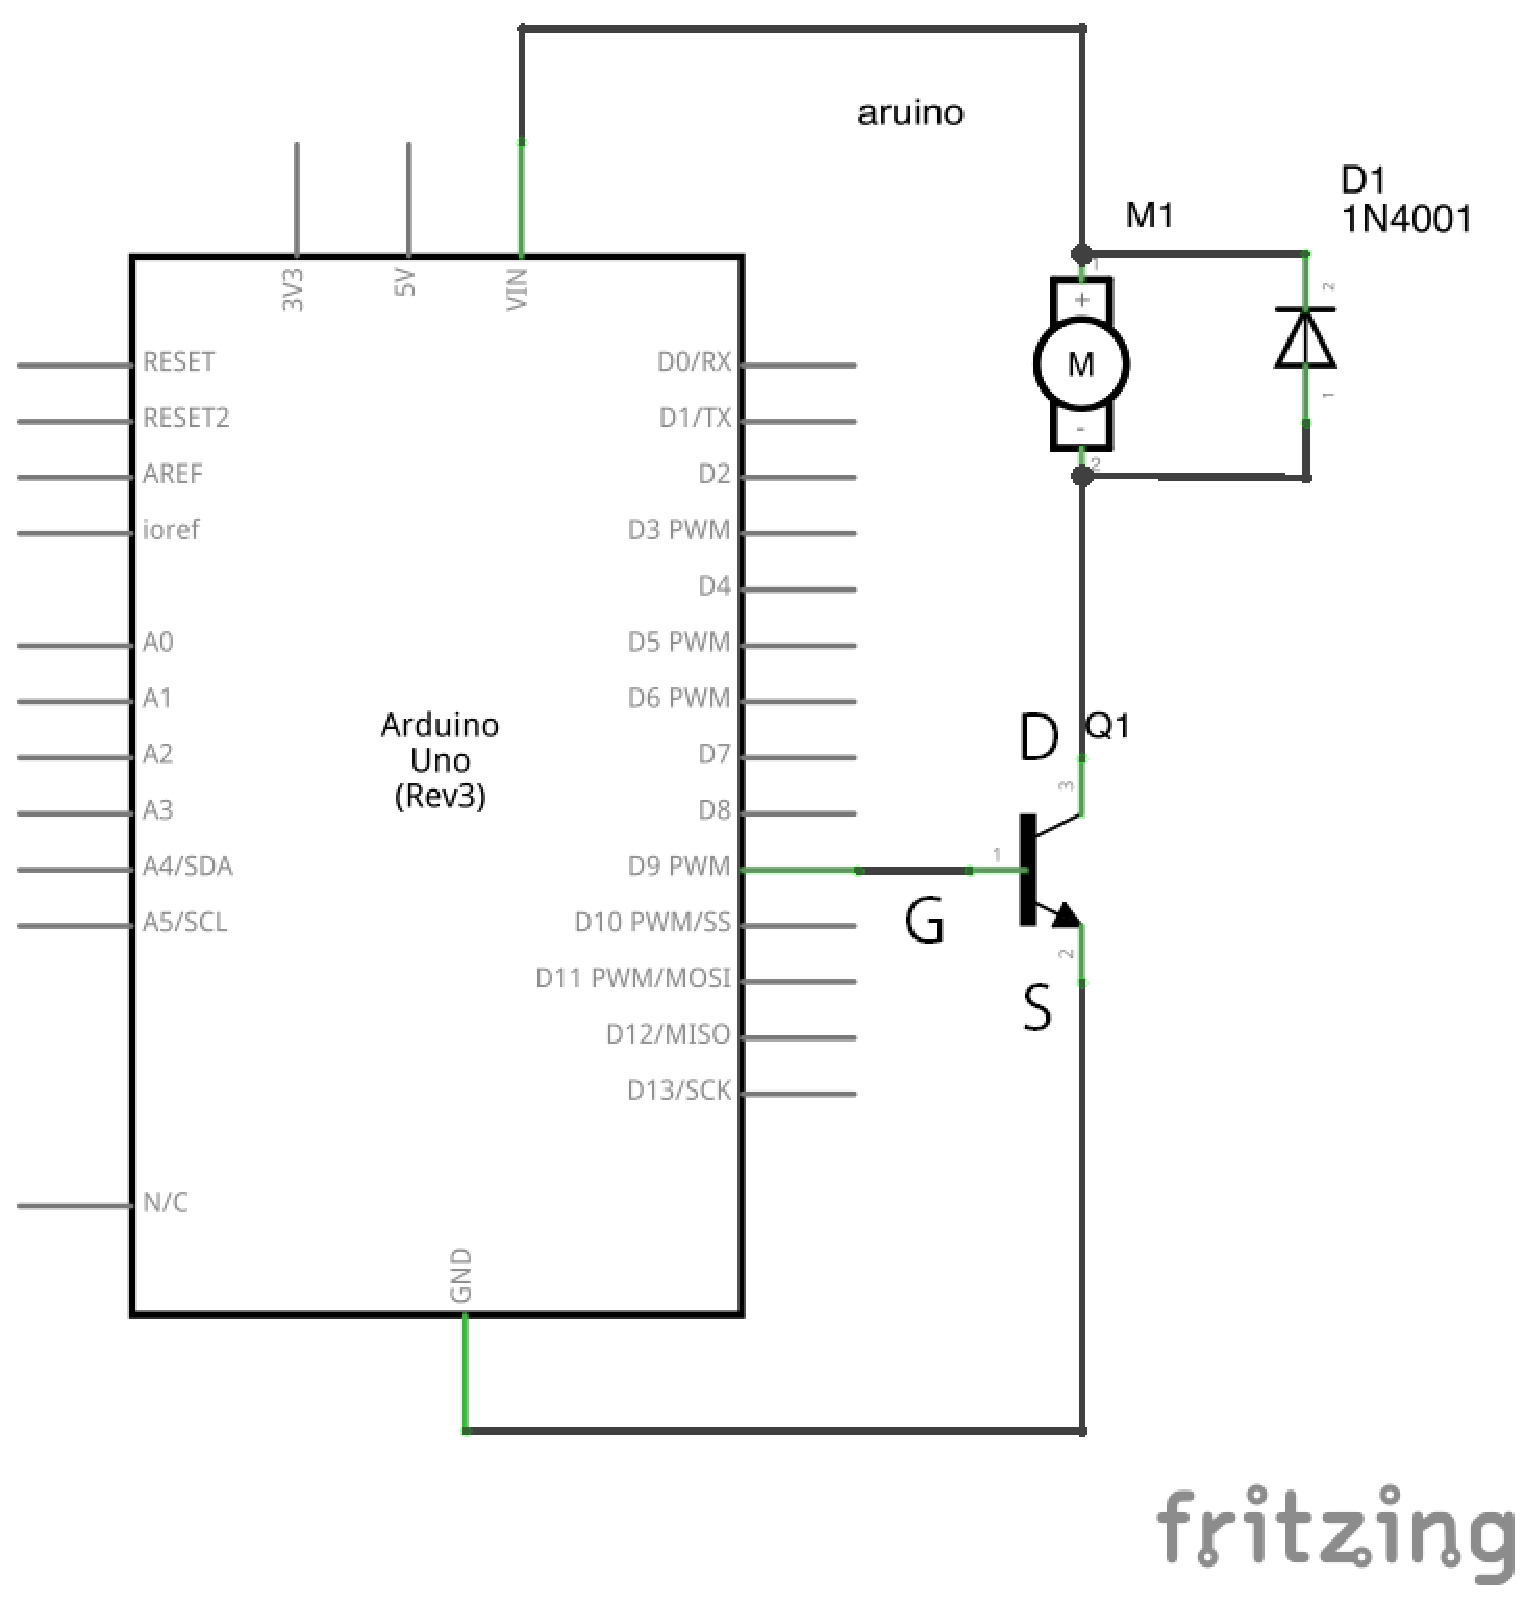
\includegraphics[width=0.5\columnwidth]{img/motor_control.eps}
 \caption{モーター制御のための回路図}
\end{figure}

\subsection*{プログラム}
\begin{lstlisting}
import processing.serial.*;
import cc.arduino.*;
 
Arduino arduino;
int MOTOR = 9;
 
void setup() {
  arduino = new Arduino(this, Arduino.list()[6], 57600);
  arduino.pinMode(MOTOR, Arduino.OUTPUT);
}
 
void draw() {
  arduino.analogWrite(MOTOR,128);
}
\end{lstlisting}

\section{赤外線センサからの入力に基づいてモーターを制御する}

\subsection*{回路}
% \begin{figure}[h!]
%  \centering
%  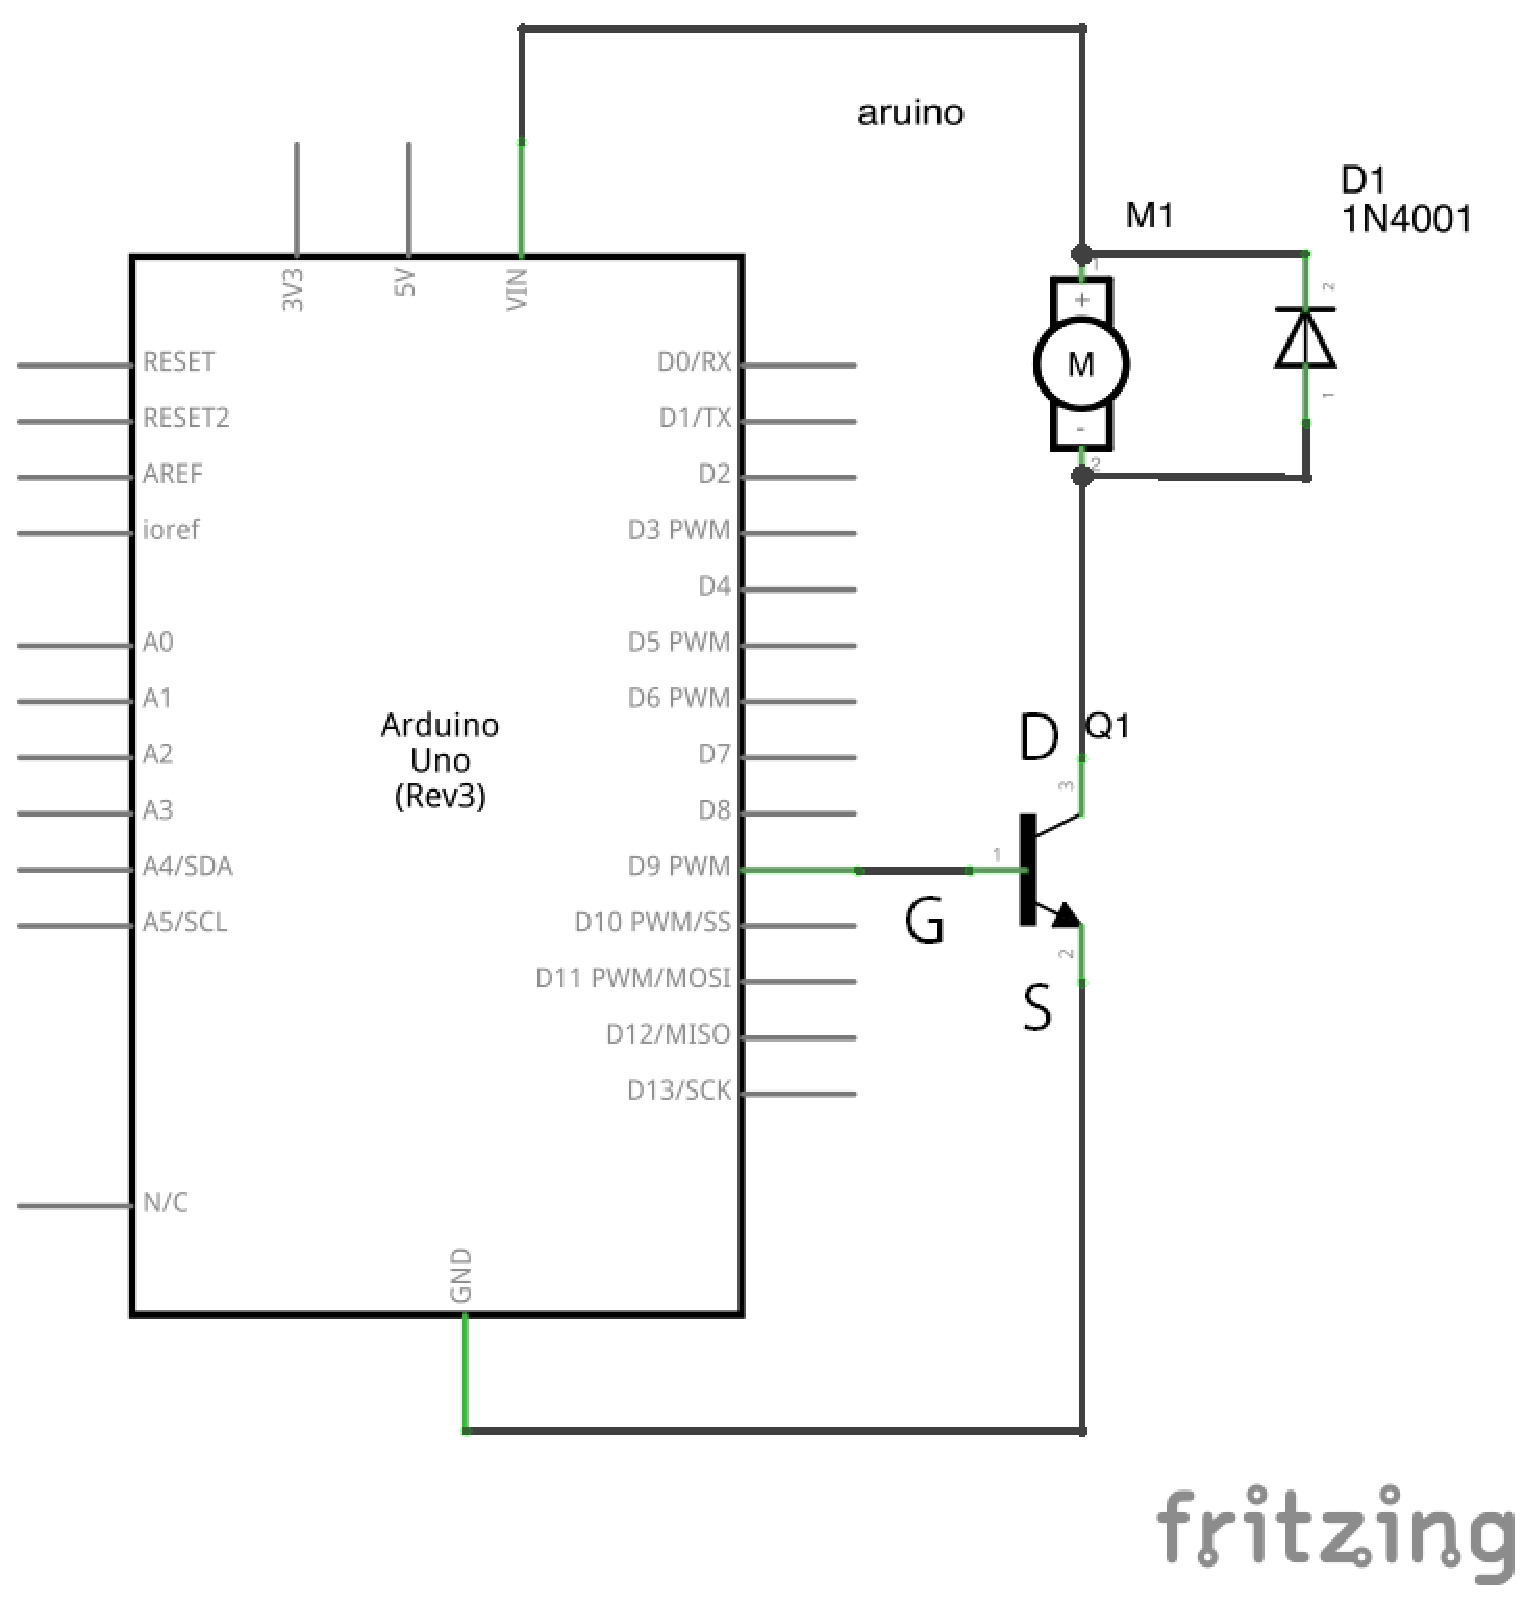
\includegraphics[width=\columnwidth]{img/motor_control.eps}
%  \caption{モーター制御のための回路図}
% \end{figure}

\subsection*{プログラム}
\begin{lstlisting}
 
\end{lstlisting}


\end{document}